\documentclass[12pt]{article}
\usepackage[utf8]{inputenc}
\usepackage{geometry}
\geometry{a4paper, margin=1in}
\usepackage{graphicx}
\usepackage{hyperref}
\usepackage{amsmath}
\usepackage{pgfplots}
\pgfplotsset{compat=1.18}

\title{Comprehensive Project 0001}
\author{Project Manager: John Doe}
\date{September 24, 2024}

\begin{document}

\maketitle

\tableofcontents
\newpage

\section{Introduction}
This comprehensive project memo provides an in-depth update on the ABC project, outlining the progress, key risks, mitigation strategies, and upcoming milestones. The memo is structured to give detailed insights into each phase of the project and highlight crucial areas of focus for the upcoming months.

The project’s goal is to increase system performance by 30\%, making it more efficient and scalable for future requirements. Since the last update in August, we have made significant progress, but challenges remain, particularly in API integration and database optimization.

\section{Project Overview}
The ABC project is divided into three phases:
\begin{itemize}
    \item \textbf{Phase 1: Requirement Gathering} (Completed)
    \item \textbf{Phase 2: Development} (Ongoing)
    \item \textbf{Phase 3: Testing and Deployment} (Scheduled)
\end{itemize}

\subsection{Phase 1: Requirement Gathering}
Phase 1 was completed on August 15, 2024. During this phase, we collaborated with key stakeholders to gather comprehensive requirements. This ensured alignment between the development team and business goals.

The requirement gathering process revealed several areas of potential improvement, including enhancing system security, scaling infrastructure to support additional users, and integrating third-party APIs to increase functionality.

\subsection{Phase 2: Development}
Phase 2, which started in mid-August, has been divided into two key workstreams: frontend development and backend integration.

\paragraph{Frontend Development} The user interface has been redesigned for improved user experience. Feedback from the design team suggests that the new UI reduces user friction, particularly in high-traffic environments.

\paragraph{Backend Integration} The backend system is undergoing significant upgrades, including:
\begin{itemize}
    \item Implementation of a microservices architecture.
    \item Enhanced database management.
    \item API integration.
\end{itemize}

We are currently facing delays in backend API integration, which has impacted the project timeline. We are, however, adding additional resources to ensure this delay does not extend into the next phase.

\section{Current Status}
As of September 24, 2024, we have made significant progress in both frontend development and backend integration.

\subsection{Progress Metrics}
The following table provides a high-level view of the project's progress, outlining the percentage completed for key components of Phase 2.

\begin{table}[h!]
\centering
\begin{tabular}{|c|c|c|}
\hline
\textbf{Component} & \textbf{Target Completion Date} & \textbf{Progress (\%)} \\
\hline
Frontend Development & October 5, 2024 & 80\% \\
Backend Development & October 20, 2024 & 60\% \\
API Integration & October 1, 2024 & 50\% \\
Database Optimization & October 10, 2024 & 70\% \\
\hline
\end{tabular}
\caption{Progress Summary for Key Components}
\end{table}

\subsection{Development Burndown Chart}
Below is a burndown chart that shows the team's progress over the last six weeks. It tracks the remaining work against the total planned work for Phase 2.

\begin{center}
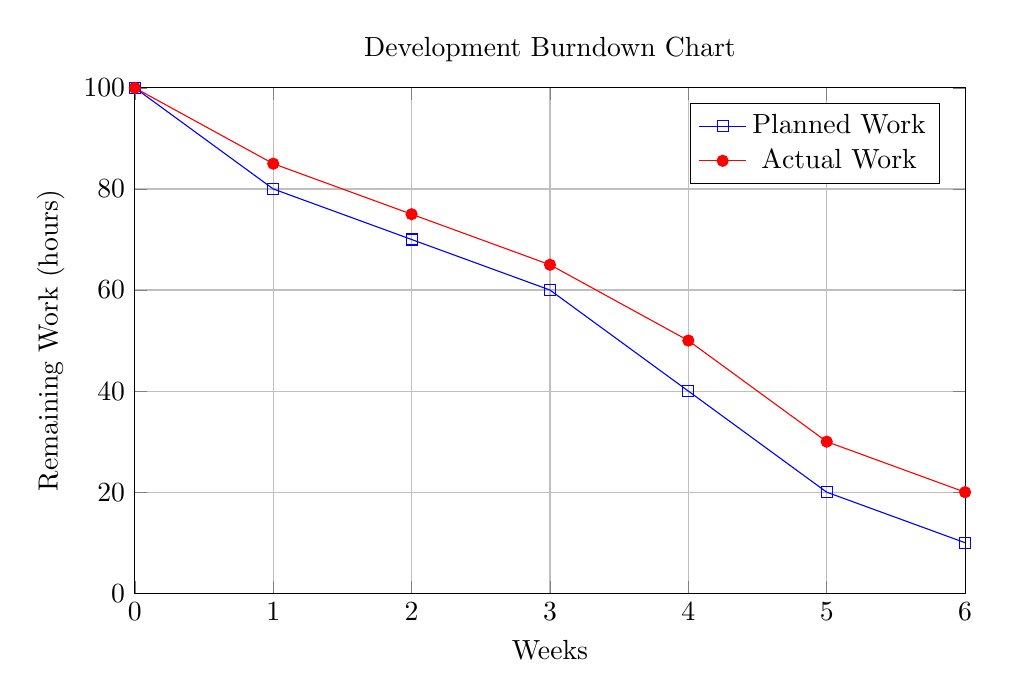
\begin{tikzpicture}
\begin{axis}[
    title={Development Burndown Chart},
    xlabel={Weeks},
    ylabel={Remaining Work (hours)},
    xmin=0, xmax=6,
    ymin=0, ymax=100,
    xtick={0,1,2,3,4,5,6},
    ytick={0,20,40,60,80,100},
    legend pos=north east,
    grid=major,
    width=\linewidth,
    height=8cm
]
\addplot[color=blue,mark=square] coordinates {
    (0, 100) (1, 80) (2, 70) (3, 60) (4, 40) (5, 20) (6, 10)
};
\addplot[color=red,mark=*] coordinates {
    (0, 100) (1, 85) (2, 75) (3, 65) (4, 50) (5, 30) (6, 20)
};
\legend{Planned Work, Actual Work}
\end{axis}
\end{tikzpicture}
\end{center}

\newpage
\section{Key Risks and Mitigation Strategies}
Several risks have been identified, with corresponding mitigation strategies outlined below:

\subsection{Risk 1: API Integration Delays}
\textbf{Description:} Delays in integrating third-party APIs have caused a bottleneck in the backend development. This may push the timeline for backend completion by two weeks.

\textbf{Mitigation Strategy:} An additional developer has been assigned to the API integration team to speed up the process. We are also in discussions with the third-party vendor to expedite the required changes.

\subsection{Risk 2: Database Scalability Issues}
\textbf{Description:} Early testing has revealed potential issues in database scalability. This could lead to performance bottlenecks when the system is under heavy load.

\textbf{Mitigation Strategy:} The architecture team is revisiting the database design. We plan to implement a horizontal scaling solution that will distribute the load across multiple database instances.

\section{Upcoming Milestones}
The next steps in the project include the following key milestones:

\begin{itemize}
    \item \textbf{October 1, 2024:} Complete API integration.
    \item \textbf{October 10, 2024:} Begin comprehensive system testing, including performance and security tests.
    \item \textbf{October 20, 2024:} Finish backend development, including database optimization.
    \item \textbf{November 5, 2024:} Start phased deployment to staging environments.
    \item \textbf{November 15, 2024:} Final deployment to production.
\end{itemize}

\section{Conclusion}
The ABC project is progressing well, although certain risks remain, particularly in API integration and database scalability. With the additional resources being allocated to the project and close collaboration with external vendors, we expect to meet the revised deadlines. A detailed status update will be provided in next month’s project memo, scheduled for October 24, 2024.

\end{document}
